% !TEX TS-program = pdflatex
% !TEX encoding = UTF-8 Unicode

% This is a simple template for a LaTeX document using the "article" class.
% See "book", "report", "letter" for other types of document.

\documentclass[11pt]{article} % use larger type; default would be 10pt

\usepackage[utf8]{inputenc} % set input encoding (not needed with XeLaTeX)

%%% Examples of Article customizations
% These packages are optional, depending whether you want the features they provide.
% See the LaTeX Companion or other references for full information.

%%% PAGE DIMENSIONS
\usepackage{geometry} % to change the page dimensions
\geometry{a4paper} % or letterpaper (US) or a5paper or....
% \geometry{margin=2in} % for example, change the margins to 2 inches all round
% \geometry{landscape} % set up the page for landscape
%   read geometry.pdf for detailed page layout information

\usepackage{graphicx} % support the \includegraphics command and options

% \usepackage[parfill]{parskip} % Activate to begin paragraphs with an empty line rather than an indent

%%% PACKAGES
\usepackage{booktabs} % for much better looking tables
\usepackage{array} % for better arrays (eg matrices) in maths
%\usepackage{paralist} % very flexible & customisable lists (eg. enumerate/itemize, etc.)
\usepackage{verbatim} % adds environment for commenting out blocks of text & for better verbatim
\usepackage{subfig} % make it possible to include more than one captioned figure/table in a single float
\usepackage{setspace} %paquete para interlineado
\usepackage{graphicx} %para insertar graficos
\usepackage{parskip} % npi de q es
\usepackage{color} %colores
\usepackage{float}


% These packages are all incorporated in the memoir class to one degree or another...

%%% HEADERS & FOOTERS
\usepackage{fancyhdr} % This should be set AFTER setting up the page geometry
\pagestyle{fancy} % options: empty , plain , fancy
\renewcommand{\headrulewidth}{0pt} % customise the layout...
\lhead{}\chead{}\rhead{}
\lfoot{}\cfoot{\thepage}\rfoot{}

%%% SECTION TITLE APPEARANCE
\usepackage{sectsty}
\allsectionsfont{\sffamily\mdseries\upshape} % (See the fntguide.pdf for font help)
% (This matches ConTeXt defaults)

%%% ToC (table of contents) APPEARANCE
\usepackage[nottoc,notlof,notlot]{tocbibind} % Put the bibliography in the ToC
\usepackage{color}
\usepackage{listings}

\usepackage[titles,subfigure]{tocloft} % Alter the style of the Table of Contents
\renewcommand{\cftsecfont}{\rmfamily\mdseries\upshape}
\renewcommand{\cftsecpagefont}{\rmfamily\mdseries\upshape} % No bold!

%%% END Article customizations

\usepackage[spanish]{babel}
\usepackage{listings} 
%%% The "real" document content comes below...
\lstset{language=html,caption={Ejemplos Basicos: Hola Mundo y otros programas introductorios},label=DescriptiveLabel}

   
\lstdefinestyle{customc}{
  belowcaptionskip=1\baselineskip,
  breaklines=true,
  frame=L,
  xleftmargin=\parindent,
  language=C,
  showstringspaces=false,
  basicstyle=\footnotesize\ttfamily,
 keywordstyle=\bfseries\color{green!40!black},
  commentstyle=\itshape\color{purple!40!black},
  identifierstyle=\color{blue},
 stringstyle=\color{red},
}


\lstset{escapechar=@,style=customc}





\title{Bucamina - Android}



\author{Fausto Mora, Christian Vergara, \\ Angel Gonzalez}
\begin{document}


%\date{} % Activate to display a given date or no date (if empty),
         % otherwise the current date is printed 

\maketitle
%\tableofcontents % No hace falta un TOC en un artículo corto

\section{Introducción}
\newcommand{\oops}[1]{\textit{#1}}

\section{Obejetivo del Proyecto}
\section{Objetivo Especificos}
\section{Descripcion}
\section{Diagramas de casos de uso }

\begin{center}
Presentacion del Diagrama de Casos de Uso del proyecto en plataforma Android.\ref{fig:casosdeusos}

	\begin{figure}[h!]
  		\centering
    		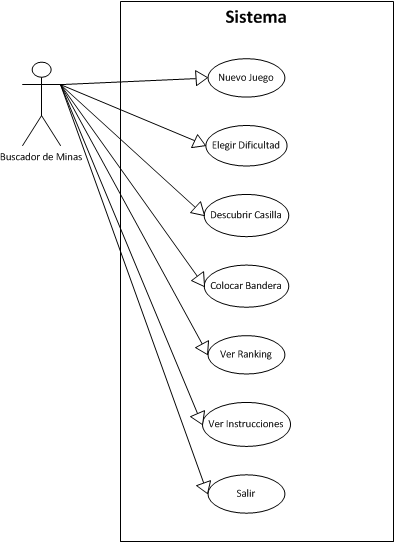
\includegraphics[width=0.3\textwidth]{imagenes/casosdeusos.png}
  		\caption{Casos de Usos}
		\label{fig:casosdeusos}
	\end{figure}
\end{center}



\section{Requisitos no funcionales }
\section{Diagrama de clases }

\begin{center}
Presentacion del Diagrama de Clases para el proyecto en plataforma Android.\ref{fig:diagclass}
\\\
	\begin{figure}[h!]
  		\centering
    		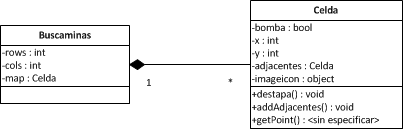
\includegraphics[width=0.7\textwidth]{imagenes/buscamina_diagclass.png}
  		\caption{Diagrama de Clases}
		\label{fig:diagclass}
	\end{figure}
\end{center}

\section{Arquitectura en Android}
\section{Conclusiones}


\end{document}
